\documentclass[polish, 9pt, xcolor=table, hyperref={pdfpagemode=FullScreen}]{beamer}

\mode<presentation>
{
  \usetheme{metropolis}
  % or ...

  \setbeamercovered{transparent}
  % or whatever (possibly just delete it)
}

\usepackage{subcaption}
\usepackage{polski}
% or whatever

\usepackage{babel}
\usepackage[utf8]{inputenc}
% or whatever

\usepackage{times}
\usepackage[T1]{fontenc}
% Or whatever. Note that the encoding and the font should match. If T1
% does not look nice, try deleting the line with the fontenc.

\usepackage{tikz}
\usetikzlibrary{cd, patterns, patterns.meta, decorations.pathmorphing}

\newcommand{\R}{\mathbb{R}}


\title[Czarne Dziury Schwarzchilda] % (optional, use only with long paper titles)
{Modelowanie horyzontów zdarzeń czarnych dziur przy użyciu metryki Schwarzchilda}

\subtitle
{Rozwiązania analityczne i numeryczne } % (optional)

\author[Aleksandra Niedziela, Weronika Jakimowicz] % (optional, use only with lots of authors)
{Aleksandra Niedziela \and Weronika Jakimowicz}
% - Use the \inst{?} command only if the authors have different
%   affiliation.

\institute[Uniwersytet Wrocławski] % (optional, but mostly needed)
{
  Wydział Matematyki i Informatyki\\
  Uniwersytet Wrocławski
 }
% - Use the \inst command only if there are several affiliations.
% - Keep it simple, no one is interested in your street address.

\date[Short Occasion] % (optional)
{22.01.2024 / Zespołowy Projekt Specjalnościowy}

\subject{Talks}
% This is only inserted into the PDF information catalog. Can be left
% out. 



% If you have a file called "university-logo-filename.xxx", where xxx
% is a graphic format that can be processed by latex or pdflatex,
% resp., then you can add a logo as follows:

% \pgfdeclareimage[height=0.5cm]{university-logo}{university-logo-filename}
% \logo{\pgfuseimage{university-logo}}



% Delete this, if you do not want the table of contents to pop up at
% the beginning of each subsection:
\AtBeginSection[]
{
  \begin{frame}<beamer>{Spis treści}
    \tableofcontents[currentsection]
  \end{frame}
}


% If you wish to uncover everything in a step-wise fashion, uncomment
% the following command: 

%\beamerdefaultoverlayspecification{<+->}


\begin{document}

\begin{frame}
  \titlepage
\end{frame}

\begin{frame}{Spis treści}
  \tableofcontents
  % You might wish to add the option [pausesections]
\end{frame}


% Since this a solution template for a generic talk, very little can
% be said about how it should be structured. However, the talk length
% of between 15min and 45min and the theme suggest that you stick to
% the following rules:  

% - Exactly two or three sections (other than the summary).
% - At *most* three subsections per section.
% - Talk about 30s to 2min per frame. So there should be between about
%   15 and 30 frames, all told.

\section{Czym są czarne dziury?}

\subsection[Czarne Dziura Schwarzchilda]{Czarne Dziury Schwarzchilda}

\begin{frame}{Czarne Dziura Schwarzchilda}
  % - A title should summarize the slide in an understandable fashion
  %   for anyone how does not follow everything on the slide itself.
\begin{columns}
\begin{column}{0.5\textwidth}
\begin{itemize}
\item
	Wyróżniamy cztery rodzaje czarnych dziur: 
\begin{itemize}
\item
	Schwarzchilda
\item 
	Kerra 
\item
	Reissner–Nordströma
\item 
	Kerra–Newmana
\end{itemize}
\item 
	Są to obiekty o nieskończonej gęstości, tak masywne, że zakrzywią czasoprzestrzeń wokół siebie.
\item 
	Powstają podczas śmierci gwiazdy w wybuchu supernowej. 
\item
	Czarne dziury są inspiracją dla wielu autorów science fiction - \textit{Interstellar}.
\end{itemize}
\end{column}
	
\begin{column}{0.5\textwidth}
\begin{figure}
\centering
 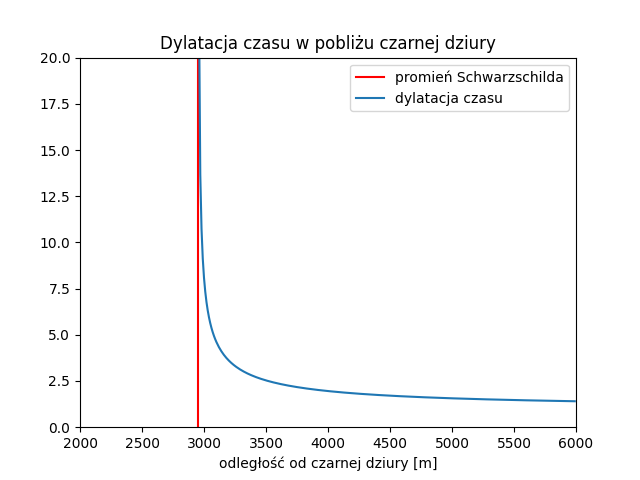
\includegraphics[width=0.7\textwidth]{ilustracje/Time_near_black_hole.png}
\end{figure}

\begin{figure}
\centering
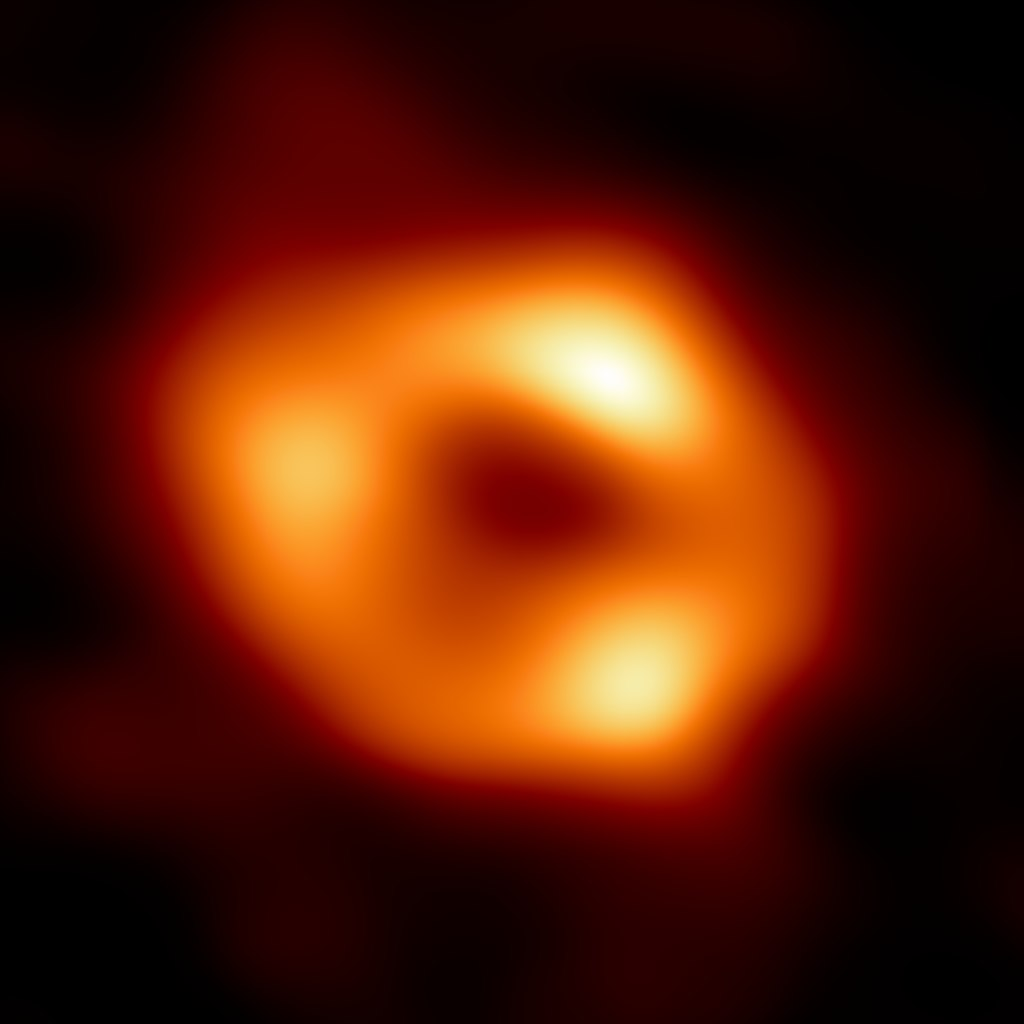
\includegraphics[width=0.5\textwidth]{ilustracje/zakazany_donut.jpg}
\end{figure}
\end{column}
\end{columns}
\end{frame}


\subsection{Czarna Dziura jako rozmaitość Riemannowska}

\begin{frame}{Czarna Dziura jako rozmaitość Riemannowska}

\textbf{Rozmaitość} to pojęcie matematyczne opisujące przestrzeń $M$, która wokół każdego punktu $p \in M$ posiada otwarte otoczenie $U_p$, które przypomina pewien podzbiór przestrzeni $\R^n$.

Schwarzchild opisywał czarną dziurę, modelując przestrzeń wokół niej jako rozmaitość różniczkowalną z tensorem metrycznym, czyli rozmaitość Riemannowską.

\begin{figure}
\centering
    \begin{subfigure}[t]{0.3\textwidth}
        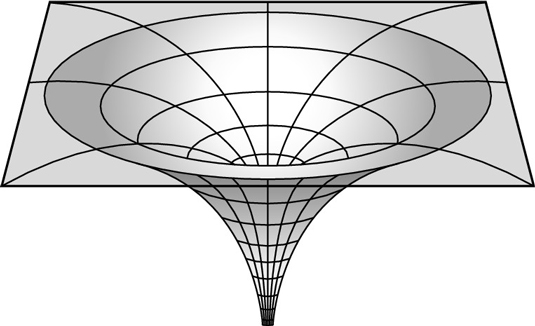
\includegraphics[width=0.7\textwidth]{ilustracje/dziura.jpg} 
    \end{subfigure}
    \begin{subfigure}[b]{0.3\textwidth}
        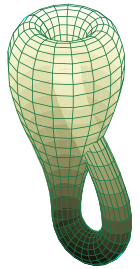
\includegraphics[width=0.5\textwidth]{ilustracje/rozmaitosc2.svg.png}
    \end{subfigure}
    \begin{subfigure}[b]{0.3\textwidth}
        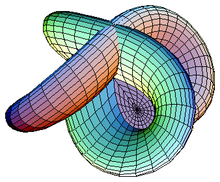
\includegraphics[width=0.7\textwidth]{ilustracje/rozmaitosc1.PNG}
    \end{subfigure}
\end{figure}

\end{frame}

\begin{frame}{Metryka Schwarzchilda}

Metryka Schwarzchilda jest zdefiniowana na podzbiorze $\R \times (0, +\infty) \times S^2$ o sygnaturze $(-, +, +, +)$, który jest standardowo zapisywany jako

$$ g = c^2 d \tau^2 = -\frac{r - r_s}{r}\cdot c^2d t^2 + \left( \frac{r - r_s}{r}\right)^{-1} d r^2 + r^2(d \theta^2 + \sin^2(\theta) d \phi^2) $$

lub w postaci macierzy:

$$
g_{\mu, \nu} = \begin{bmatrix}
  -\frac{1 - r_s}{r}\cdot c^2 & 0                               & 0   & 0 \\
  0                 & \left(\frac{1 - r_s}{r}\right)^{-1} & 0   & 0 \\
  0                 & 0                                   & r^2 & 0 \\ 
  0                 & 0                                   & 0   & r^2 \sin^2(\theta)
\end{bmatrix}, 
$$

\end{frame}

\section{Proste ścieżki na zakrzywionych powierzchniach}

\subsection{Linie geodezyjne}

\begin{frame}{Proste ścieżki na zakrzywionych powierzchniach}

Foton podróżując po przestrzeni wokół czarnej dziury nie przyspiesza, tzn. druga pochodna krzywej opisującej jego trasę jest stale równa zero.

$$\frac{d^2 \gamma} {d t^2}=0.$$ 

Cząstka będzie szukać najszybszej (najkrótszej) drogi między dwoima punktami - takiej która pochłonid najmniej energii. Na rozmaitości nazywamy ją \textbf{linią geodezyją}

\renewcommand{\figurename}{Rysunek}
\begin{figure}
  \centering 
  \vspace{1cm}
  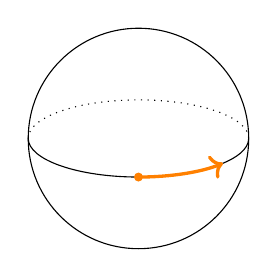
\begin{tikzpicture}[scale = 0.7] 
    \draw (0, 0) circle (2);
    \draw (-2, 0) arc (180:360:2 and 0.7);
    \draw[dotted] (-2, 0) arc (180:0:2 and 0.7);

    \draw[very thick, ->, orange] (0, -0.7) arc (270:320:2 and 0.7);
    \filldraw[orange] (0, -0.7) circle (2pt);
  \end{tikzpicture}
  \caption{Cząsteczka poruszająca się po sferze $S^2$.}\label{czasteczka po sferze}
  \vspace{1cm}
\end{figure}

\end{frame}

\subsection{Koneksja Levi-Civity}

\begin{frame}{Koneksja Levi-Civity}

Wraz z fotonem przesuwamy przestrzeń styczną, jednak powoduje to pewne problemy.

\begin{figure}[h]
  \centering 
	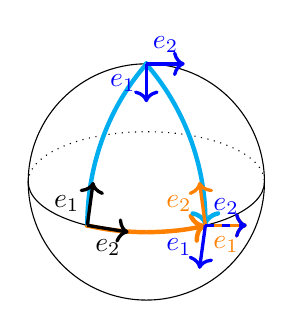
\begin{tikzpicture}[scale = 0.5]
    \draw (0, 0) circle (3);
    \draw (-3, 0) arc (180:360:3 and 1.275);
    \draw[dotted] (-3, 0) arc (180:0:3 and 1.275);

    \draw[orange, ultra thick, ->] (0, -1.275) arc (270:300:3 and 1.275);
    \draw[orange, ultra thick] (0, -1.275) arc(270:240:3 and 1.275);

    \filldraw[orange] (-1.5, -1.1025) circle (1.5pt);
    \filldraw[orange] (1.5, -1.1025) circle (1.5pt);

    \draw[cyan, ultra thick] (-1.5, -1.1025) arc (180:135:5.25 and 5.85);
    \draw[cyan, ultra thick, <-] (1.5, -1.1025) arc (0:45:5.25 and 5.85);

    \filldraw[cyan] (0, 3) circle (1.5pt);

    \draw[->, very thick] (-1.5, -1.1025)--(-1.35, 0) node [midway, left] {$e_1$};
    \draw[->, very thick] (-1.5, -1.1025)--(-0.45, -1.275) node [midway, below] {$e_2$};

    \draw[->, very thick, blue] (0, 3)--(0.975, 3) node [midway, above] {$e_2$};
    \draw[->, very thick, blue] (0, 3)--(0, 2.025) node [midway, left] {$e_1$};

    \draw[->, very thick, orange] (1.5, -1.1025)--(1.35, 0) node [midway, left] {$e_2$};
    \draw[->, very thick, orange] (1.5, -1.1025)--(2.55, -1.1025) node [midway, below] {$e_1$};
    
    \draw[->, very thick, blue, dashed] (1.5, -1.1025)--(2.55, -1.1025) node [midway, above] {$e_2$};
    \draw[->, very thick, blue] (1.5, -1.1025)--(1.35, -2.205) node [midway, left] {$e_1$};
  \end{tikzpicture}

\end{figure}

By uzgodnić jak będziemy przesuwać przestrzeń styczną wzdłóż krzywej potrzebne jest użycie koneksji Levi-Civity, dla której definiujemy \textbf{symbole Christofela} jako liczby, spełniające równanie:

$$ \nabla_j \partial_k=\Gamma_{j k}^l \partial_l. $$

\end{frame}

\section{Matematyczna podróż do czarnej dziury}

\subsection{Symbole Christofela}

\begin{frame}{Wyliczenie Symboli Christofela}

Zamiast liczyć symbole Christofela wprost z definicji możemy skorzystać z lagrangianu:

$$ S = \int L d \lambda $$

Dla metryki Schwarzchilda mamy:

$$ S = \int d \tau= \int \frac{d \tau}{d \tau} d \tau = \int \frac{\sqrt{d \tau^2}}{d \tau} d \tau = \int \sqrt{g_{\mu, \nu}\dot{x^\mu} \dot{x^\nu}}d \tau = \int L' d \tau. $$

Korzystamy również z równań Eulera-Lagrange'a

$$\frac{d}{ d \tau}\left(\frac{\partial L}{\partial \dot{x^\mu}}\right)= \frac{\partial L}{\partial x^\mu}\; . $$

\end{frame}

\begin{frame}{Wyliczenie Symboli Christofela}

Otrzymujemy układ równań:

\begin{align*}
  \ddot{t}&=-\frac{1}{r(r-1)}\dot{r}\dot{t}\\
  \ddot{r}&=-\frac{r-1}{ 2r^3} \dot{t}^2+\frac{1}{2r(r-1)}\dot{r}^2+(r-1)\dot{\theta}^2+(r-1)\sin^2\theta \dot{\phi}^2\\
  \ddot{\theta} &= \sin \theta \cos \theta \dot{\phi}^2 - \frac{2}{ r} \dot{r}\dot{\theta}\\
  \ddot{\phi} &= -\frac{2}{r} \dot{r}\dot{\phi} - 2 \frac{\cos \theta}{ \sin \theta} \dot{\phi}  \dot{\theta} 
\end{align*}

\end{frame}

\begin{frame}{Wyliczenie Symboli Christofela c.d}

Z których wyliczmamy symbole Christofela:

\begin{align*}
  \Gamma_{t,r}^t&=\frac{1}{2r(r-1)}\\ 
  \Gamma_{t,t}^r&=\frac{r-1}{2r^3}\\ 
  \Gamma_{r,r}^r&=-\frac{1}{2r(r-1)}\\ 
  \Gamma_{\phi,\phi}^r&=-(r-1)\\ 
  \Gamma_{r,\phi}^\phi&=\frac{1}{r} 
\end{align*}

\end{frame}

\subsection{Równanie orbity}

\begin{frame}{Równanie orbity}

Korzystamy jeszcze raz z równań Eulera-Langrange'a, dostajemy

$$ \frac{d}{d\tau}(2r^2\dot{\phi})=0 $$
$$ \frac{d}{d\tau}\left(2\frac{r-1}{r}\dot{t}\right)=0 $$

Dzięki temu możemy wyliczyć równanie orbity:

\begin{align}
  \left(\frac{du}{d\phi}\right)^2&=\frac{1}{b^2}-u^2+u^3\label{rownanie_orbity}\\ 
  u'' &=u\left(\frac{3}{2}u-1\right)\label{zmiana predkosci}
\end{align}

\end{frame}

\begin{frame}{Ścieżki fotonów}

Rozwiązując równanie orbity dzięki funkcji  \texttt{odeint} z biblioteki \texttt{scipy} języka Python otrzymujemy:

\begin{figure}[h]
  \centering
  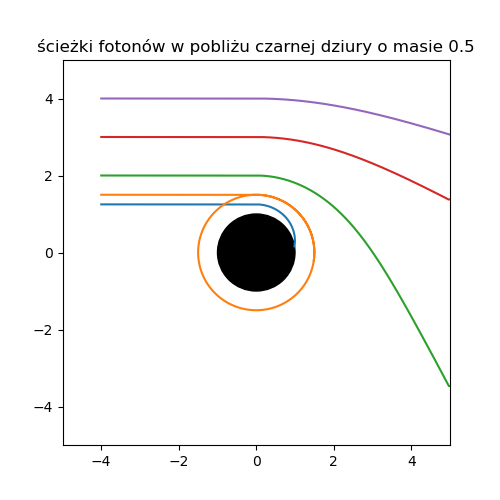
\includegraphics[width=0.5\textwidth]{ilustracje/sceizki_wykres.png}
  \caption{Ścieżki fotonów w pobliżu czarnej dziury o masie $M=\frac{1}{2}$ i promieniu Schwarzschilda $r_s=1$ ($c=1=G$) uzyskane przy pomocy języka Python.}
\end{figure}

\end{frame}

\end{document}


